
\documentclass[aspectratio=169]{beamer}
\usetheme{Madrid}
 
\usepackage{graphicx}
%\usepackage[spanish]{babel}
\usepackage[utf8]{inputenc}
\usepackage{hyperref}
\usepackage{verbatim}

\usepackage[linesnumbered,lined,commentsnumbered]{algorithm2e}

%\setbeamertemplate{footline}[frame number]

\begin{document}


\title{Introduction to neural networks}  
\subtitle{Warren McCulloch \& Walter Pitts Model} 
\author[J.I. Vasquez]{\textbf{Juan Irving Vásquez} \\jivg.org}
\date{\today \copyright}
\institute[jivg.org]{Centro de Innovación y Desarrollo Tecnológico en Cómputo \\ Instituto Politécnico Nacional}
% logo of my university
\titlegraphic{
\includegraphics[height=1.2cm]{ipn-cidetec.png}\hspace{0.1cm}
\includegraphics[height=1.2cm]{escudoESCOM}}
\frame{\titlepage} 

%%%%%%%%%%%%%%%%%%%%%%%%%%%%%%%%%%%%%%%%%%%%%%%%%%%%%%%%

\frame{
	\frametitle{Contents}
\tableofcontents
}


\begin{frame}
\frametitle{The big picture \footnote{https://medium.com/@lmpo/a-brief-history-of-ai-with-deep-learning-26f7948bc87b}}
\centering
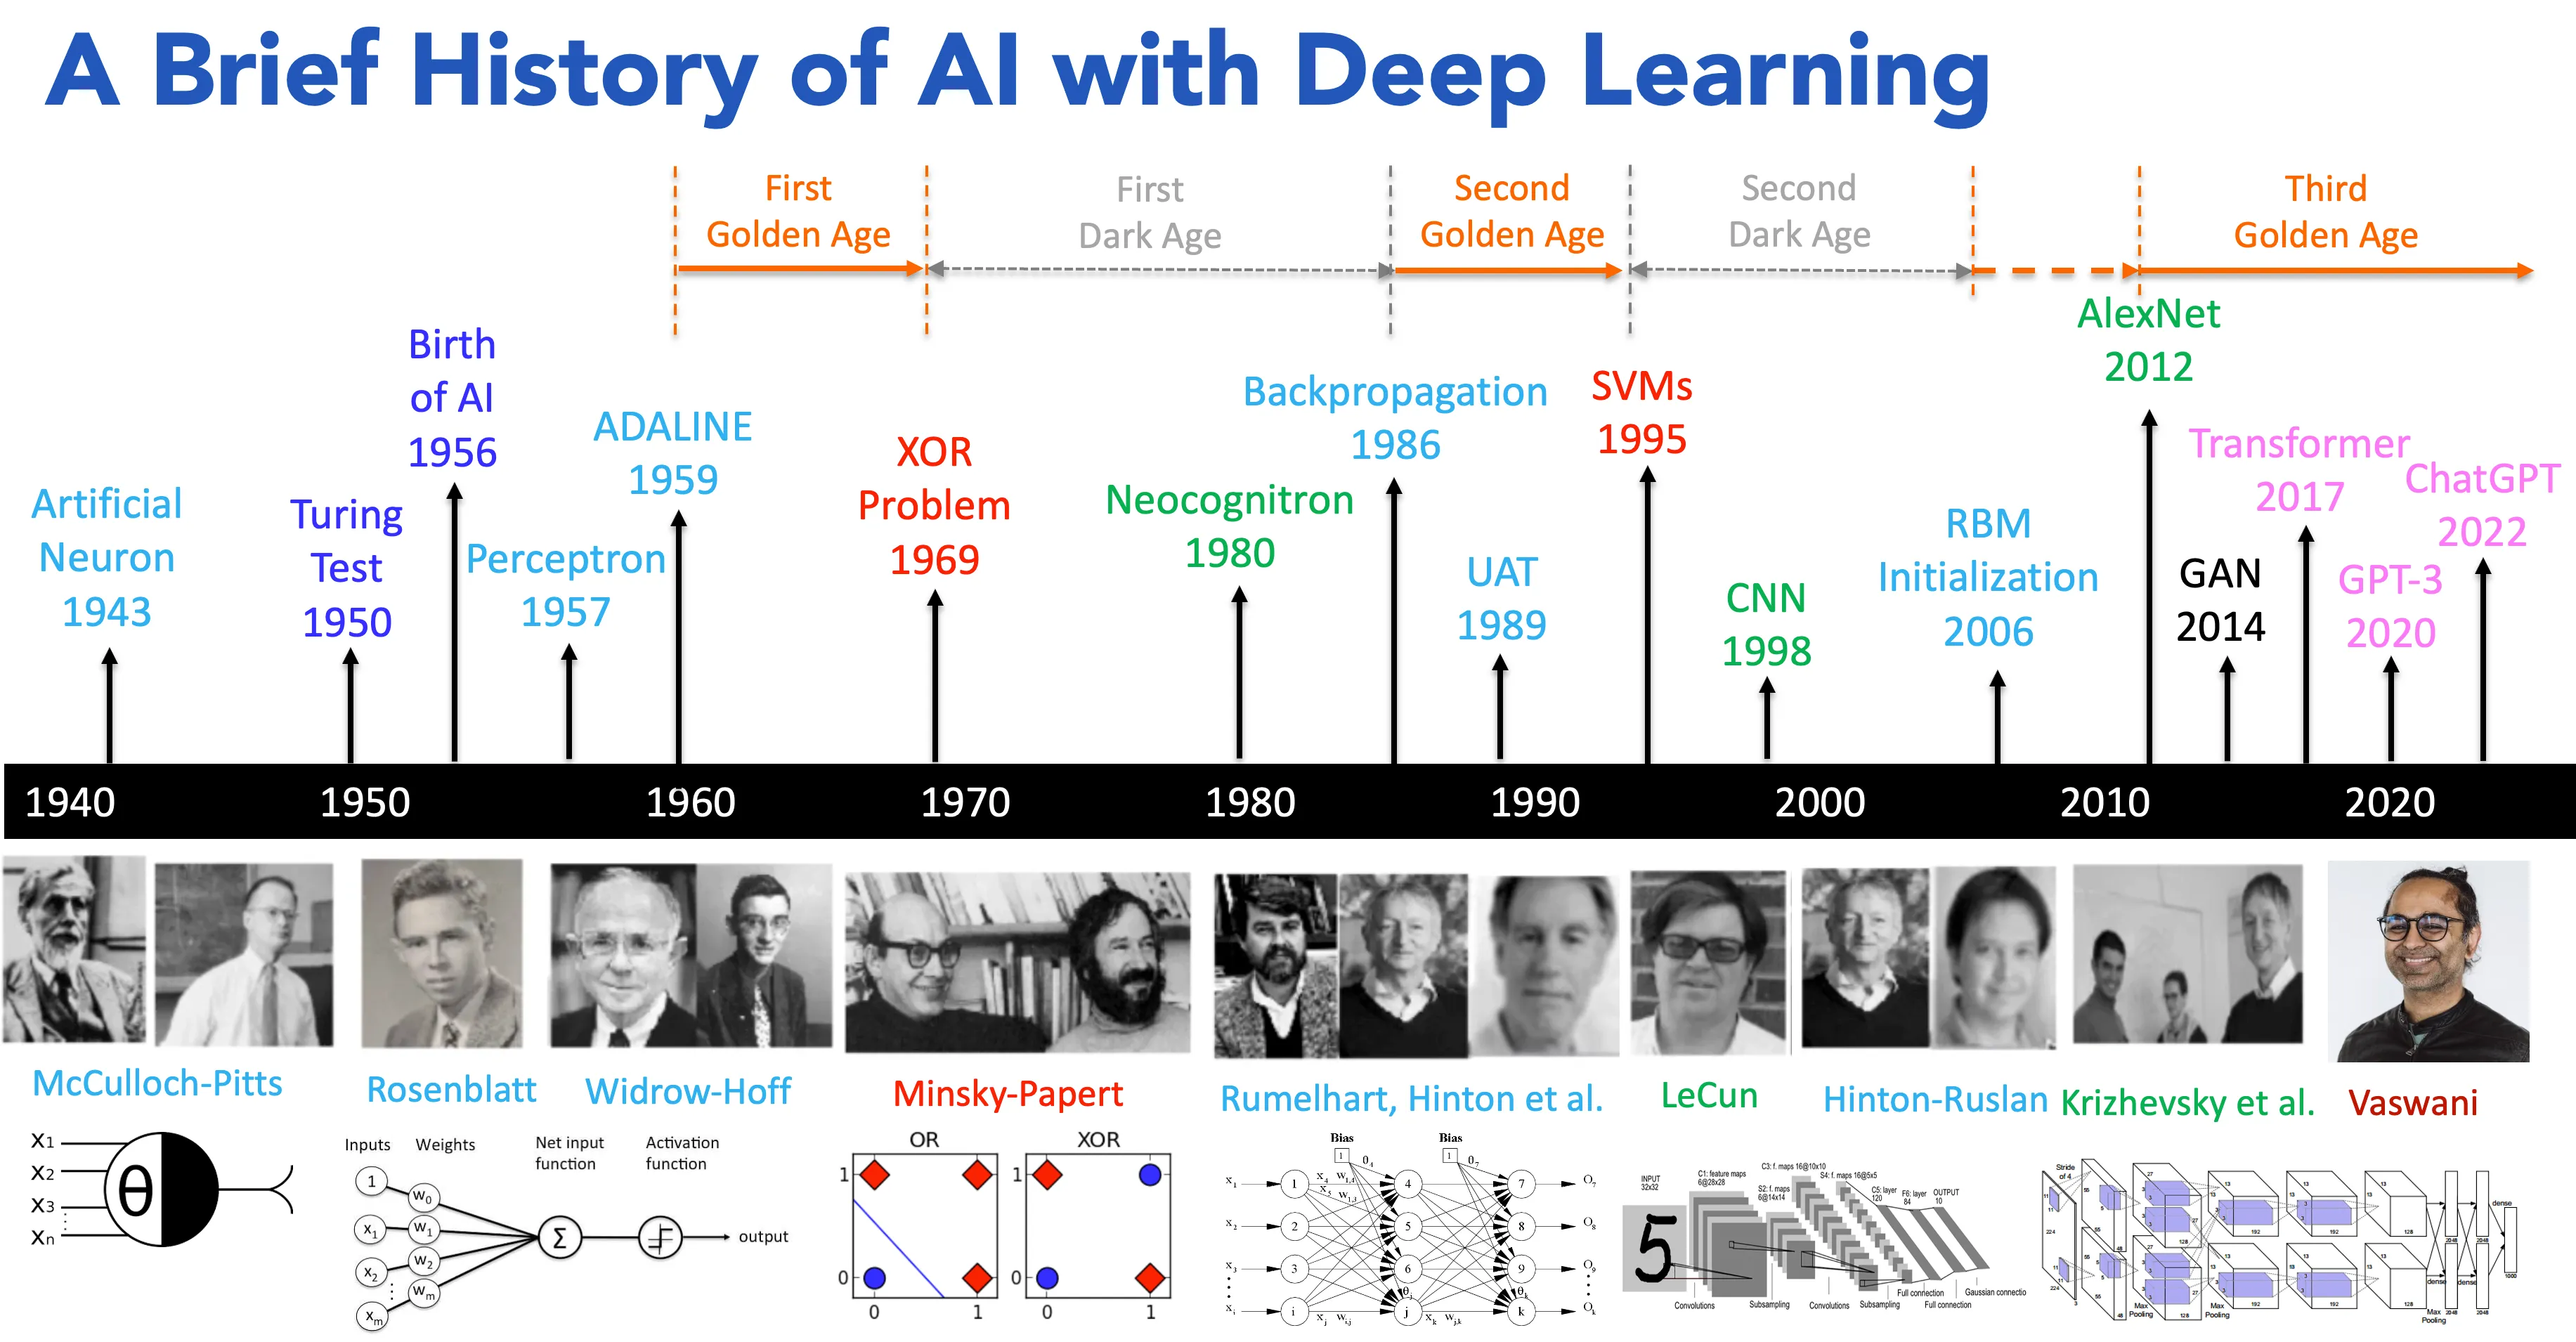
\includegraphics[trim={0 0 0 190},clip,width=0.92\textwidth]{timeline}
\end{frame}


\begin{frame}
\frametitle{The problem}
\begin{itemize}
	\item Conexionism: replicate the human intelligence by simulating the brain funcioning.
	\item The base of a brain: the neuron.
	\item Given an input $X \in \mathbb{B}^n$, build a machine, $f$, that check if the input is similar to a target signal, namely.
	\begin{equation}
		y = f(X)?
	\end{equation}
\end{itemize}
\end{frame}


\section{Warren McCulloch \& Walter Pitts Model}

\frame{
	\frametitle{Warren McCulloch \& Walter Pitts}
	\begin{figure}
		\centering
		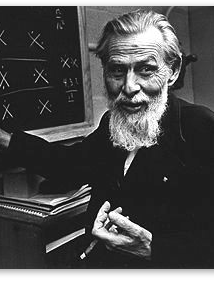
\includegraphics[height=0.69\textheight]{wmc_1}
		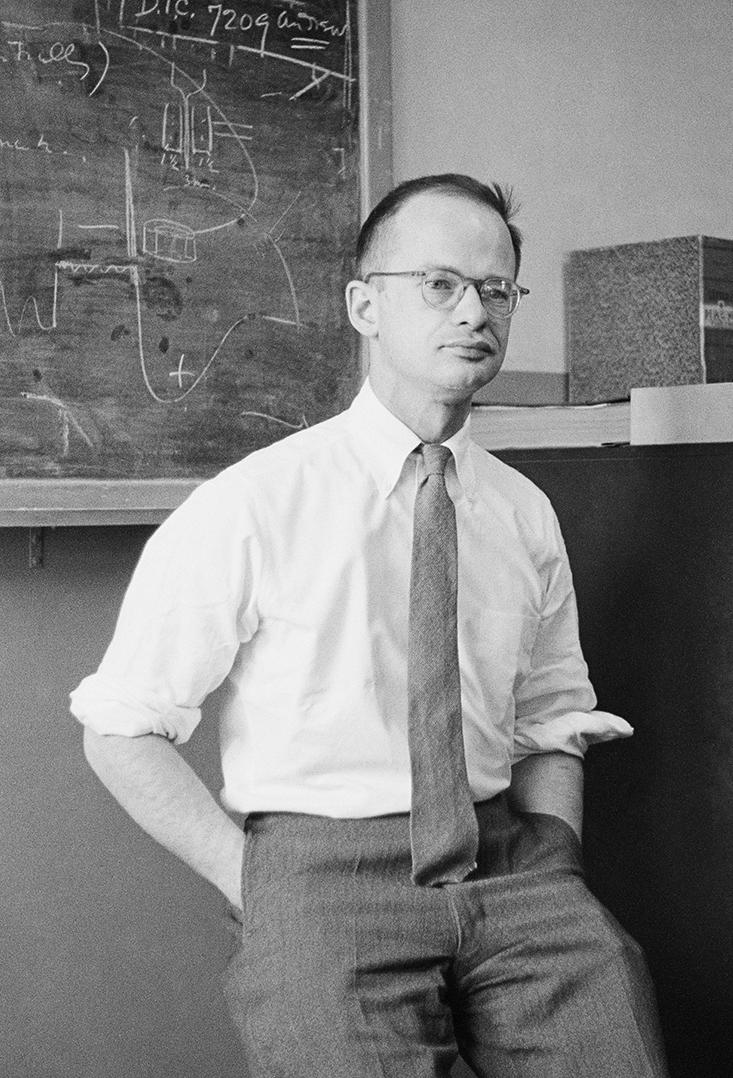
\includegraphics[height=0.69\textheight]{wp}
		\caption{Warren McCulloch and Walter Pitts\footnote{\url{https://es.wikipedia.org/wiki/Walter_Pitts}}}
		\label{fig:0925rosenblattmain}
	\end{figure}
}

\begin{frame}
\frametitle{A littie bit of history}
\begin{itemize}
	\item Warren Sturgis McCulloch (1898-1969) \footnote{https://archives.library.illinois.edu/the-cybernetics-thought-collective-a-history-of-science-and-technology-portal-project/warren-s-mcculloch/}
	\begin{itemize}
		\item He earned his bachelor’s degree in psychology from Yale University in 1921
		\item He joined the University of Illinois Chicago in 1941 
	\end{itemize}
	\item Walter Harry Pitts (1923-1969) \footnote{Smalheiser, Neil R. "Walter pitts." Perspectives in Biology and Medicine 43.2 (2000): 217-226.}
	\begin{itemize}
		\item Assisted to the university of Chicago
		\item At the age of 15, he had read the Principia Mathematica
		\item He moved to the MIT
	\end{itemize}
\end{itemize}
\end{frame}


\begin{frame}
\frametitle{The McCulloch-Pitts model \footnote{Minsky, Marvin Lee. Computation. Chapter 3. Englewood Cliffs: Prentice-Hall, 1967}}
A neuron can be modeled as function
\begin{equation}
  \hat{y} = C(E,I,u)
\end{equation} where
exitatory input $E = \{e_1, \dots, e_n \}$, $e \in \{0,1\}$,  $I = \{\iota_1, \dots, \iota_m \}$, $i \in \{0,1\}$ and $u$ is a threshold.
\end{frame}


\begin{frame}
\frametitle{Diagram}
\begin{figure}
	\centering
	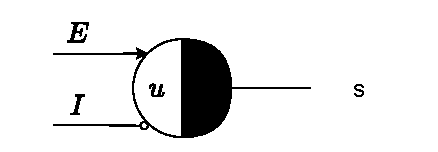
\includegraphics[width=0.7\linewidth]{myp_neuron_general.drawio}
	\caption{MyP graphical representation.}
	\label{fig:mypneurongeneral}
\end{figure}
\end{frame}


\begin{frame}[fragile]
\frametitle{Inference}
\begin{algorithm}[H]
	\SetAlgoLined
	\KwData{$E = \{e_1, \dots, e_n \}$, $I = \{\iota_1, \dots, \iota_m \}$, $u$}
	\KwResult{$\hat{y}$}
	%$\texttt{Inicializar}(W)$\tcc*{Inicializar pesos}
	\uIf{$\exists i_i = 1; i \in I$}{
		\KwRet{$0$}
	}
	\Else{
		$s = \sum_{i=1}^{n} e_i$
		\uIf{$s \geq u$}{
			\KwRet{1}
		}
		\Else{
			\KwRet{0}
		}
	}

	\label{al:modelo_myp}
	\caption{Algoritmo de inferencia de una neurona de McCulloch y Pitts.}
\end{algorithm}
\end{frame}


\begin{frame}
\frametitle{Exercises}
\begin{enumerate}
\item Dibuje el diagrama de la neurona $C=(E=\varnothing, I=\{\iota_1 \}, u = 0)$.
\item Calcule la tabla de salidas de una neurona de MyP definida por las entradas $E=[e_1], I = [\iota_1]$ y un un umbral $u = 1$.
\end{enumerate}
\end{frame}

\begin{frame}
\frametitle{On the capabilities \footnote{Hassoun, Mohamad H. Fundamentals of artificial neural networks. MIT press, 1995.}}
\begin{itemize}
\item The MyP model is considered as a linear thresholding gate (LTG).
\item A LTG belongs to the Thresholding gates group.
\item Capabilities of the LTG:
\begin{block}{LTG capabily}
Any boolean function of $n$ variables can be realized using a two-layer network with at most $2^{n-1}$ AND gates in the first (hidden layer) and a single OR gate in the second (output) layer.
\end{block}
\end{itemize}
\end{frame}


\begin{frame}
\frametitle{Further readings}
\begin{itemize}
	\item Obligatorias:
	\begin{itemize}
		\item Carroll, L. (2024). Las aventuras de Alicia en el país de las maravillas. \textbf{capítulo 6: Cerdo y pimienta.} Chibalete Editores.	
	\end{itemize}
\item Adicionales:
	\begin{itemize}
		\item Minsky, Marvin Lee. Computation. Chapter 3: NEURAL NETWORKS. AUTOMATA MADE UP OF PARTS, Englewood Cliffs: Prentice-Hall, 1967.
	\end{itemize} 
\end{itemize}
\end{frame}


\frame{
	\frametitle{References}

	\begin{itemize}
		\item Minsky, Marvin Lee. Computation. Englewood Cliffs: Prentice-Hall, 1967.
		\item Juan Irving Vasquez, \textit{Introducción a las redes neuronales}. \url{https://github.com/irvingvasquez/libro_redes_neuronales}
		\item Minsky, Marvin Lee. \textit{Computation}, Englewood Cliffs: Prentice-Hall, 1967.
		\item Image:  https://ib.bioninja.com.au/standard-level/topic-6-human-physiology/65-neurons-and-synapses/neurons.html
	\end{itemize}
}

\end{document}